%\chapter{det-comp}


%%%%%%%%%%%%%%%%%%%%%%%%%%%%%%%%%%%%%%%%%%%%%%
%\section{Anode Plane Assemblies}

%%%%%%%%%%%%%%%%%%%%%%%%%%%%%%%%%%%%%%%%%%%%%%
%\section{Cathode Plane Assemblies}

%%%%%%%%%%%%%%%%%%%%%%%%%%%%%%%%%%%%%%%%%%%%%%
\section{Field Cage (FC)}
\label{detcompsec-fc}
%%%%%%%%%%%%%%%%%%%%%%%%%
%\subsection{Scope, Requirements and Design Parameters}
\subsection{Scope and requirements} 
\fixme{Add scope}

In the TPC, each pair of facing cathode and anode planes forms an electron-drift region. A field
cage (FC) must completely surround the four open sides of this region to provide the necessary boundary
conditions to ensure a uniform electric field within, unaffected by the presence of the cryostat walls.


The FC is required to:
\begin{itemize}
\item provide the nominal drift field of 500V/cm;
\item withstand $-$180kV near the cathode;
\item define the drift distance between the APAs and CPAs to <1~cm;
\item limit the electric field in the LAr volume to under 30~kV/cm;
\item miminize the peak energy transfer in case of a HV discharge anywhere on the field cage or cathode;
\item provide redundancy in the resistor divider chain;
\item maintain the divider current much greater than the ionization current in the TPC drift cell, yet less than the power supply current limit when all dividers are connected in parallel;
\item be modular in form such that they can be easily installed in the cryostat;
\item provide support for the beam plug; \fixme{The beam plug is not defined anywhere in this document; it is just referred to several times}
\item support a 200-lb. person standing on the support beam of the bottom field cage module; and
\item prevent any trapped volume of liquid.
\end{itemize}

%%%%%%%%%%%%%%%%%%%%%%%%%
\subsection{Mechanical design}

The FC has six top and six bottom FC assemblies, arranged three along each horizontal edge of the two drift regions. It has 
four end-wall panels, one at each vertical edge of the two drift regions, see Figure~\ref{fig:fc-overview} and~\ref{fig:fc-endwall_module}.
Each endwall panel consists of four assemblies in ``landscape'' orientation, stacked vertically.
FC assemblies are constructed from pultruded G10 I-beams and box beams that support extruded field-shaping aluminum profiles. The support structure for each of the top and bottom FC assemblies consists of two main I-beams that are 3.6~m long, and three cross I-beams that brace the main I-beams for structural stability. The main I-beams have cutouts to hold the field-shaping profiles. 



\begin{cdrfigure}[An end wall field cage module]{fc-endwall_module}{A view of an end wall field cage module}
%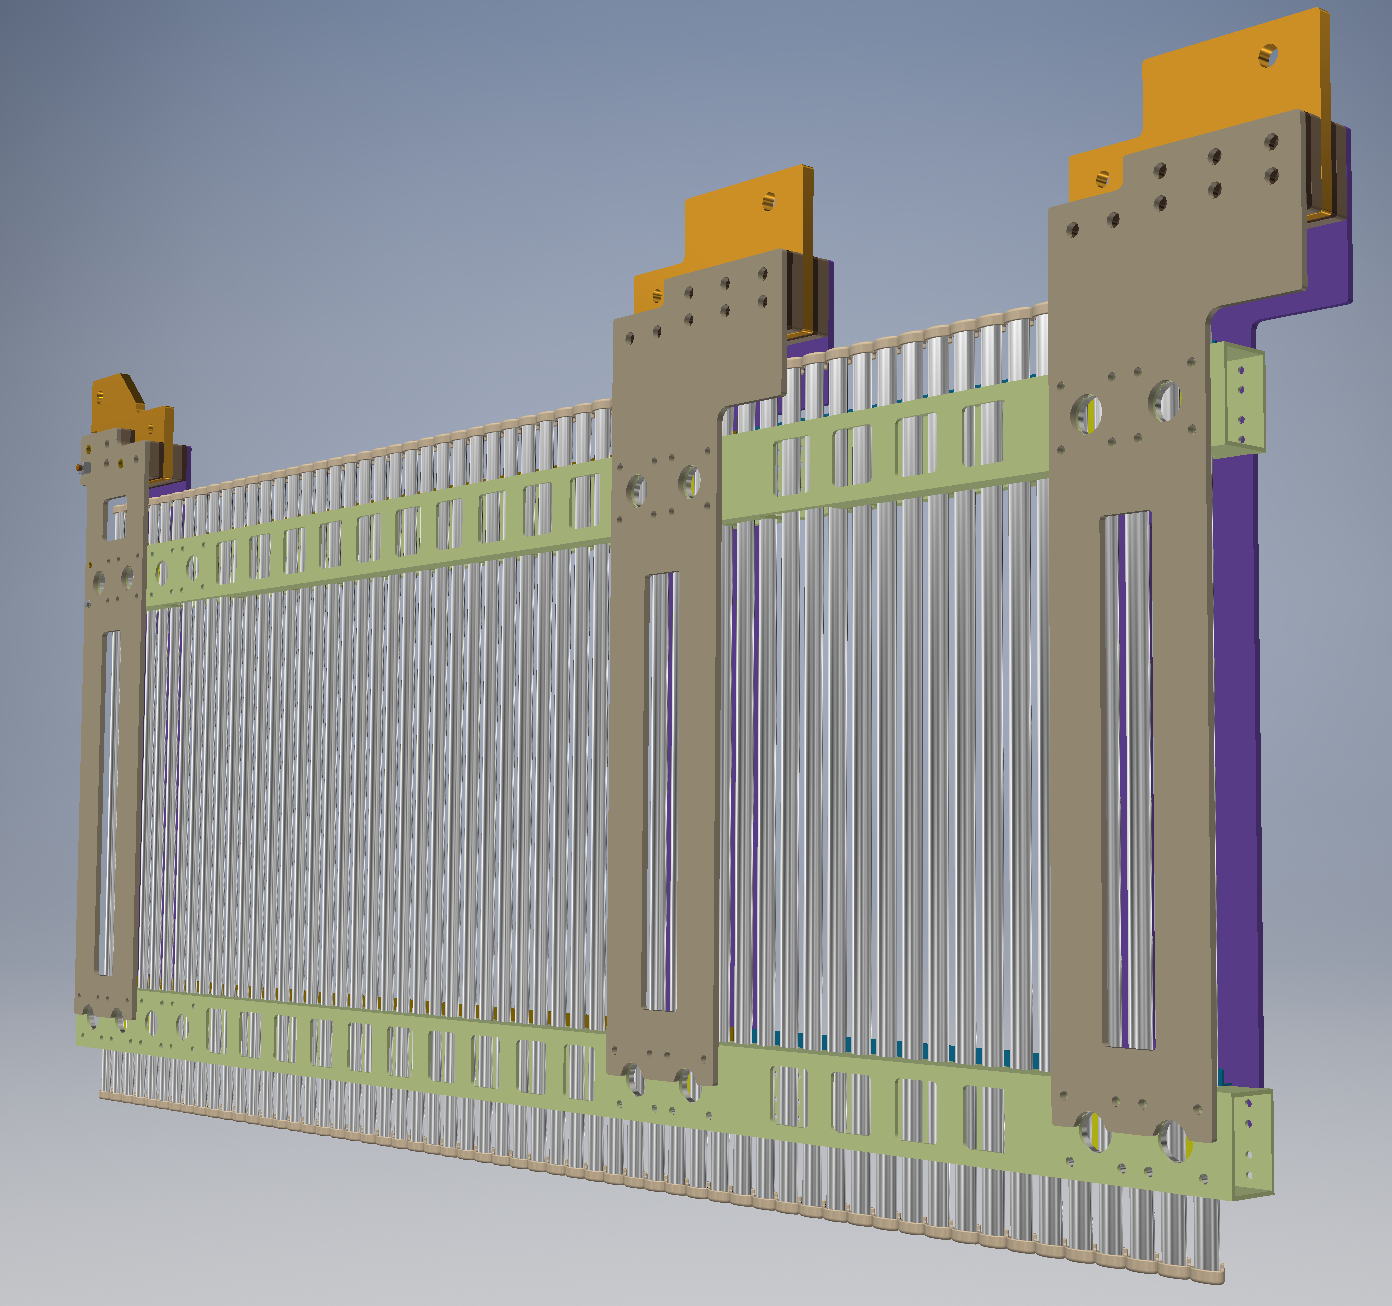
\includegraphics[width=0.6\linewidth]{tpc_fc_endwall_module.png}
\end{cdrfigure}


Aside from the profiles themselves, the nuts and bolts holding them, and the ground planes, all FC components are made of insulating material. The material selected for these structural components is fiberglass-reinforced plastic (FRP), which prevents binding when the structure is at cryogenic temperatures. The ground planes are made of stainless steel. 

The inward-facing face of the ground planes are approximately 20~cm away from the top of the field-shaping profiles. The ground planes are mounted at a fixed distance from the field shaping profiles by standoffs, as shown in Figure~\ref{fig:fc-with-ground-planes}, which shows ground planes over I-beams and cross beams.

\begin{cdrfigure}[The field cage with ground planes]{fc-with-ground-planes}{The field cage with ground planes}
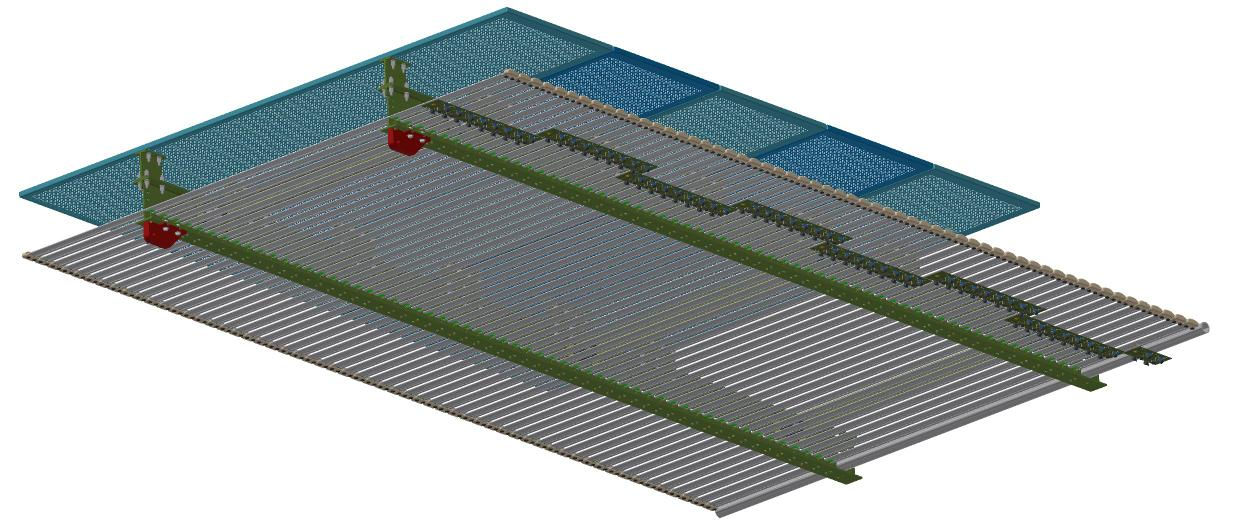
\includegraphics[width=0.8\linewidth]{fc-with-ground-planes}
\end{cdrfigure}

The parallel metal profiles in each FC assembly 
 are interconnected by a resistive divider chain, and supported by the FRP beams that span the drift distance.  Between adjacent field cage assemblies, however,  
the metal profiles are neither mechanically nor electrically connected. Gaps between assemblies that range from a few millimeters to a few centimeters are designed into the TPC assembly to ensure sufficient clearance for the installation.  The electrical isolation between the field cage modules minimizes the peak energy dump in case of a HV discharge.


%%%%%%%%%%%%%%%%%%%%%%%%%
\subsection{Electrical design}

Given a large standoff distance between the FC and the grounded cryostat wall, it is relatively easy to design a FC that meets the 30-kV/cm E field limit with 180-kV bias.  However, It becomes challenging to reduce the clearance between the FC and ground in order to make more efficient use of liquid argon.  This requires an electrode with a low profile, rounded edges, no trapped volume, and low cost.  Several commercially available roll-formed metal profiles were studied and appear to meet these requirements. \fixme{what's challenging about it then?}

Figure~\ref{fig:fc-schematic} is a schematic of the electrical design of  the CPA and a top/bottom field cage module pair.

\begin{cdrfigure}[Field cage schematic diagram]{fc-schematic}{A schematic diagram of the CPA and a top/bottom field cage module pair}
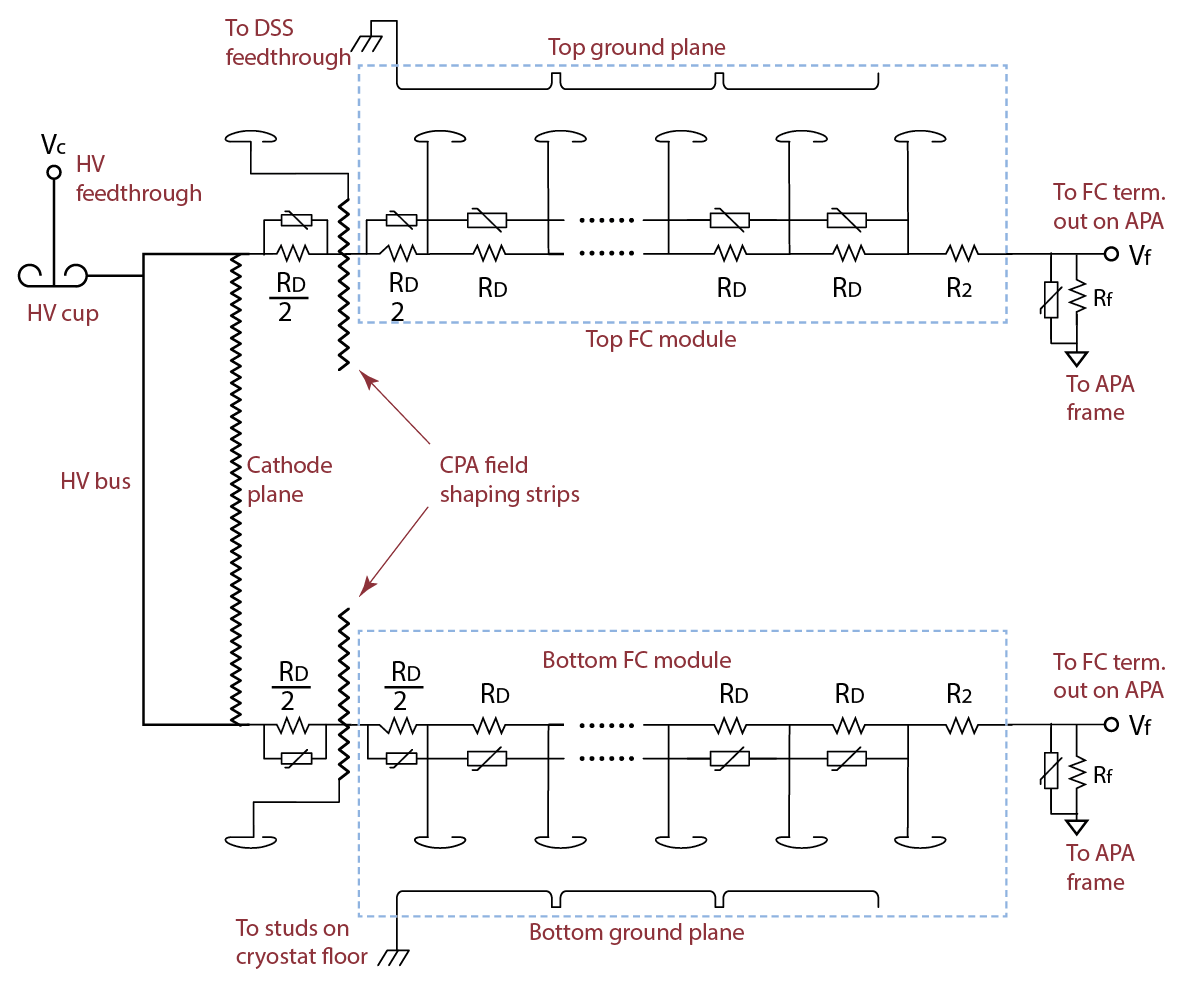
\includegraphics[width=0.8\linewidth]{tpc_fc_schematic.png}
\end{cdrfigure}




%%%%%%%%%%%%%%%%%%%%%%%%%
\subsection{FC and GP modules}

In order to confine the electric field in the liquid argon region, a grounded metallic plane is installed between the upper field cage module and the liquid-gas interface. 
Each of the six top FC modules is attached to six ground plane (GP) panels, aligned 
along their long (2,318-mm) dimension. The planes are connected to the FC beam with additional 
G10 pieces that are also used to connect adjoining GP panels. Figure~\ref{fig:c-panel-endwall-frame} shows a top/bottom FC panel with the frame and 
Figure~\ref{fig:fc_full} shows a 3D model of one fully assembled FC+GP module.

\begin{cdrfigure}[Top/bottom FC panel with endwall frame]{fc-panel-endwall-frame}{A top/bottom FC panel with the frame}
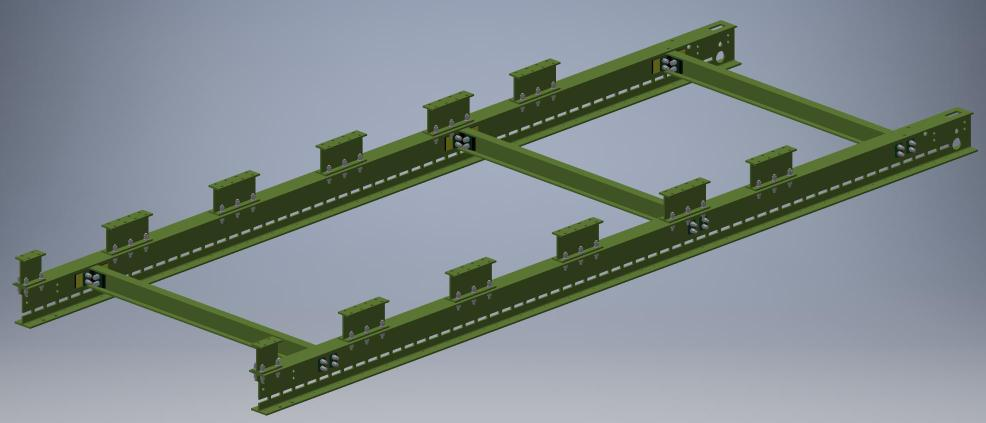
\includegraphics[width=0.8\linewidth]{fc-panel-endwall-frame}
\end{cdrfigure}

\begin{cdrfigure}[3D model of one fully assembled FC+GP module]{fc_full}{3D model of one fully assembled FC+GP module}
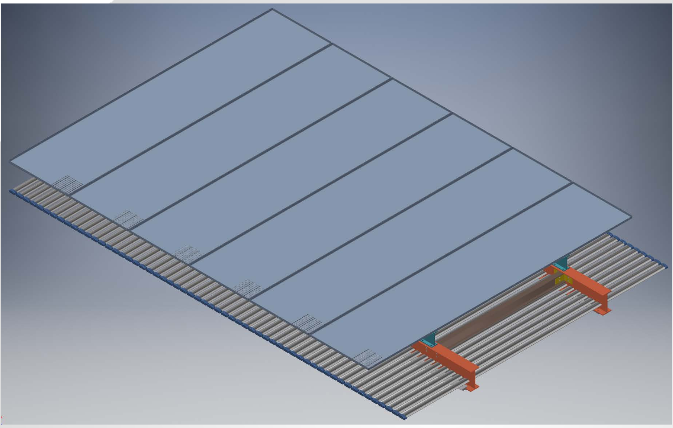
\includegraphics[width=0.8\linewidth]{tpc_topFC.png}
\end{cdrfigure}

The electrical continuity between consecutive panels can be made 
with metallic screws (with holes on the planes edges) or with looser connections, e.g., copper strips, that better adapt to the shrinking of the structure during cooldown. 
As for most detector systems, the GP is  referenced to the detector ground, located at the cryostat top.

The GP panels are installed on their corresponding (top) FC modules in the clean room outside the cryostat. %, to facilitate the connections. 
The description of how the top/bottom FC modules are assembled and connected to the CPA before insertion in the cryostat is provided in Section  \fixme{need to find and add reference}.

Further GP panels need to be attached to the top FC module:
\fixme{This little list needs work. Not clear which FC modules are intended or what these smaller GP panels are like compared to the other GP panels. Anne}
\begin{itemize}
\item Smaller panels have to be connected on the modules on one side of the CPA so that, once in position, they 
cover the CPA frame. Their dimensions are 
still to be defined, depending on the final design of the CPA hanging scheme. Such \fixme{the same pieces are connected, or similar ones are?} pieces should also be connected to the modules covering the opposite drift region, when in final position.
\item An additional 
set of small panels should be installed on the outer modules of the FC to extend the GP over the vertical FC walls, which will  
further constrain the electric field in these regions. A FEA 
shows that the optimized overhang distance is 20~cm, provided LAr is at 40~mm above the bottom of the GP. The maximal residual field in this configuration is of the order of 13~kV/cm, with less than 1~kV/cm field in the gas phase.
\end{itemize}

%%%%%%%%%%%%
\subsection{Interfaces to other TPC components}

\subsubsection{FC to CPA}

On the top and bottom of the TPC, hinges connect each field cage module to two CPA columns.  This design allows the FC modules to be pre-attached to the CPAs during installation, and prevents accidental damage to the APA wire plane when raising the field cage module to connect 
to the APA.

The end-wall field cage modules are hung from the CPA and APA support rails.  They do not have strong mechanical coupling to the CPAs and APAs, however, at least four resistive divider chains must be connected to the CPA's HV bus. \fixme{clarify how HV bus and FC are related, I'm sure it's explained elsewhere, but this sentence feels unconnected to FC. Anne}

\begin{cdrfigure}[CPA to field cage connection]{cpa-fc-connection}{A top field cage module (grey) connected to two CPA modules (brown)}
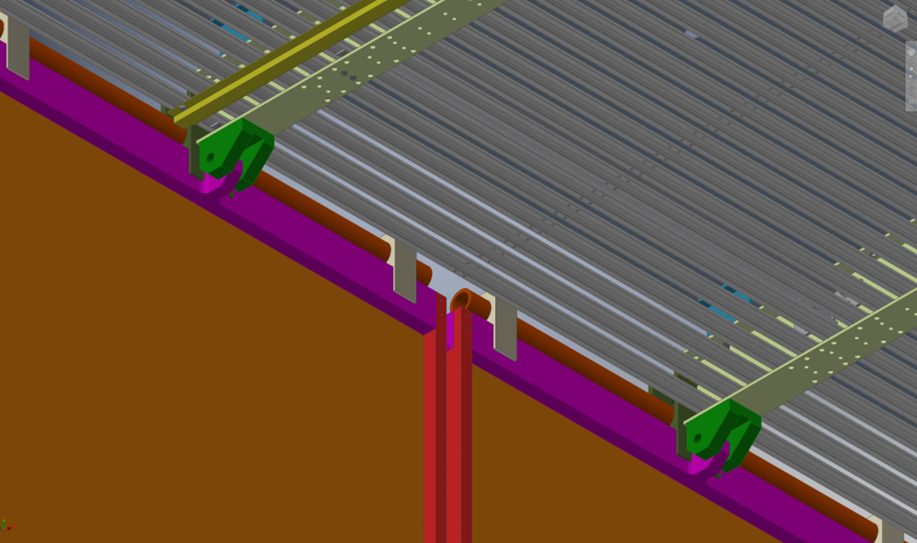
\includegraphics[width=0.8\linewidth]{tpc_fc_cpa_connection.png}
\end{cdrfigure}


%%%%%%%%%%%%
\subsubsection{FC to APA}

The I-beams of the top/bottom field cage modules are designed to be latched onto the mating brackets on the APAs.  The design details are currently being developed.   
In addition to the mechanical connection, the ground side of the divider chain must be connected to the APA's frame ground. 

\fixme{Can we get a drawing or photo of this?}

%%%%%%%%%%%%
\subsubsection{FC to beam plug}
\label{subsec:fc-beamplug}

The beam plug is designed to displace the passive LAr layer between the TPC field cage and the inner cryostat membrane. 
\fixme{displace how?}As illustrated in Figure~\ref{fig:beamplug}, it is a cylidrical glass-fiber composite pressure vessel about 50cm in length and  22cm in diameter. It is filled with dry nitrogen gas via a stainless steel line that extends to the top of the cryostat. The pressure inside the beam plug is maintained externally up to 25 psi from room to LAr temperatures. A pressure relief valve (or burst disk) is installed on the nitrogen fill line on the top of the cryostat (externally) to ensure the pressure inside the beam plug does not exceed the safety level. The component-level view of the beam plug is shown in Figure~\ref{fig:beamplug_components}.  The beam plug is secured to the field cage support structure as described in Section~\ref{subsec:fc-beamplug}. The front portion of the beam plug extends 5~cm beyond the profiles to inside the active region of the TPC through an opening on the field cage. The field cage support is designed with sufficient strength and stiffness to support the weight of the beam plug while it is suspended in air. 
When the cryostat is filled with LAr, the beam plug is roughly neutrally buoyant.  The total internal volume of the beam plug is about 16 liters. 

The requirements on the acceptable leak rate is between $7.8\times 10^{-5}$ scc/s to $15.6\times 10^{-5}$ scc/s. This is a very conservative leak rate and is roughly equivalent to 15\% of the nitrogen in the beam plug leaked over a period of a year.
  In a worst case scenario with all the nitrogen in the beam plug leaking into the LAr cryostat, the increase in concentration is about 0.1 ppm, which is still a factor of 10 below the acceptable level as specified by light detection requirements.
  \fixme{need some reference with details for this requirement}
  At nominal operation, the voltage difference across the beam plug (between the first and the last grading ring) is 165kV. 
  To minimize risk of electrical discharges, the beam plug is divided into sections and each section is bonded to stainless steel conductive grading rings. The grading rings are connected in series with two parallel path of resistor chains. There are 7 grading rings. The ring that is closest to the field cage is electrically connected to one of the field cage profiles. 
  The last ring near the cryostat wall is grounded to the stainless steel membrane via a short grounding cable. 
  The type and value of the resistor is still under evaluation. A likely candidate is the high voltage Super Mox 15G$\Omega$ resistor by OHMITE. The maximum total power dissipated by the resistor chain is about 0.6W.


\begin{cdrfigure}[Beam plug]{beamplug}{The beam plug is a  composite pressure vessel filled with dry nitrogen gas. The vessel is about 50cm in length and about 22cm in diameter. The pressure vessel is divided into sections with each section bonded to a stainless steel grading ring. The grading rings are connected by two parallel paths of resistor chain.}
  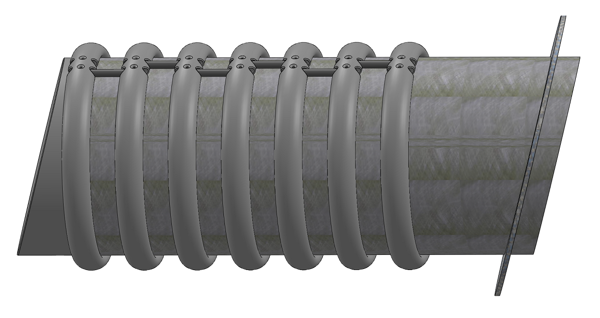
\includegraphics[width=0.6\textwidth]{beamplug.png}
\end{cdrfigure}

\begin{cdrfigure}[Beam plug component-level view]{beamplug_components}{Component-level view of the beam plug showing alternating electrode and composite ring structure.}
  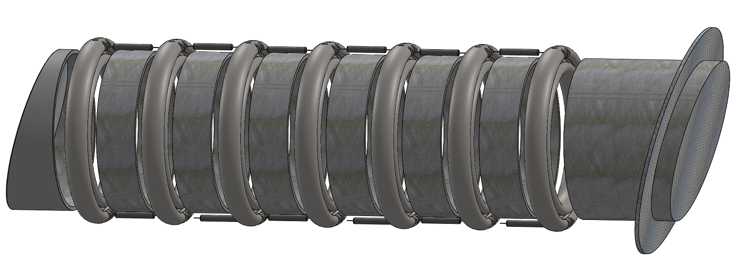
\includegraphics[width=0.7\textwidth]{beamplug_components.png}
\end{cdrfigure}

The metal electrode rings are spaced at regular intervals and interspersed with composite tube sections. The shape of the rings has been designed to minimize high electric field corners. The results of the field calculations are shown in Figures~\ref{fig:beamplug_ring1} and~\ref{fig:beamplug_ring2}. The average field in the vicinity of the beam plug is about 4.4 kV/cm. The maximum field of 15.7 kV/cm is on the electrode ring surface. In all regions the field is well below the 30 kV/cm limit.
\fixme{citation to doc describing limit would be good}

\begin{cdrfigure}[Beam plug electrodes]{beamplug_ring1}{Electric field calculation of the electrode ring design. The average field in the beam plug region is about 4.4 kV/cm. The maximum field of 15.7 kV/cm is on the electrode ring surface. }
  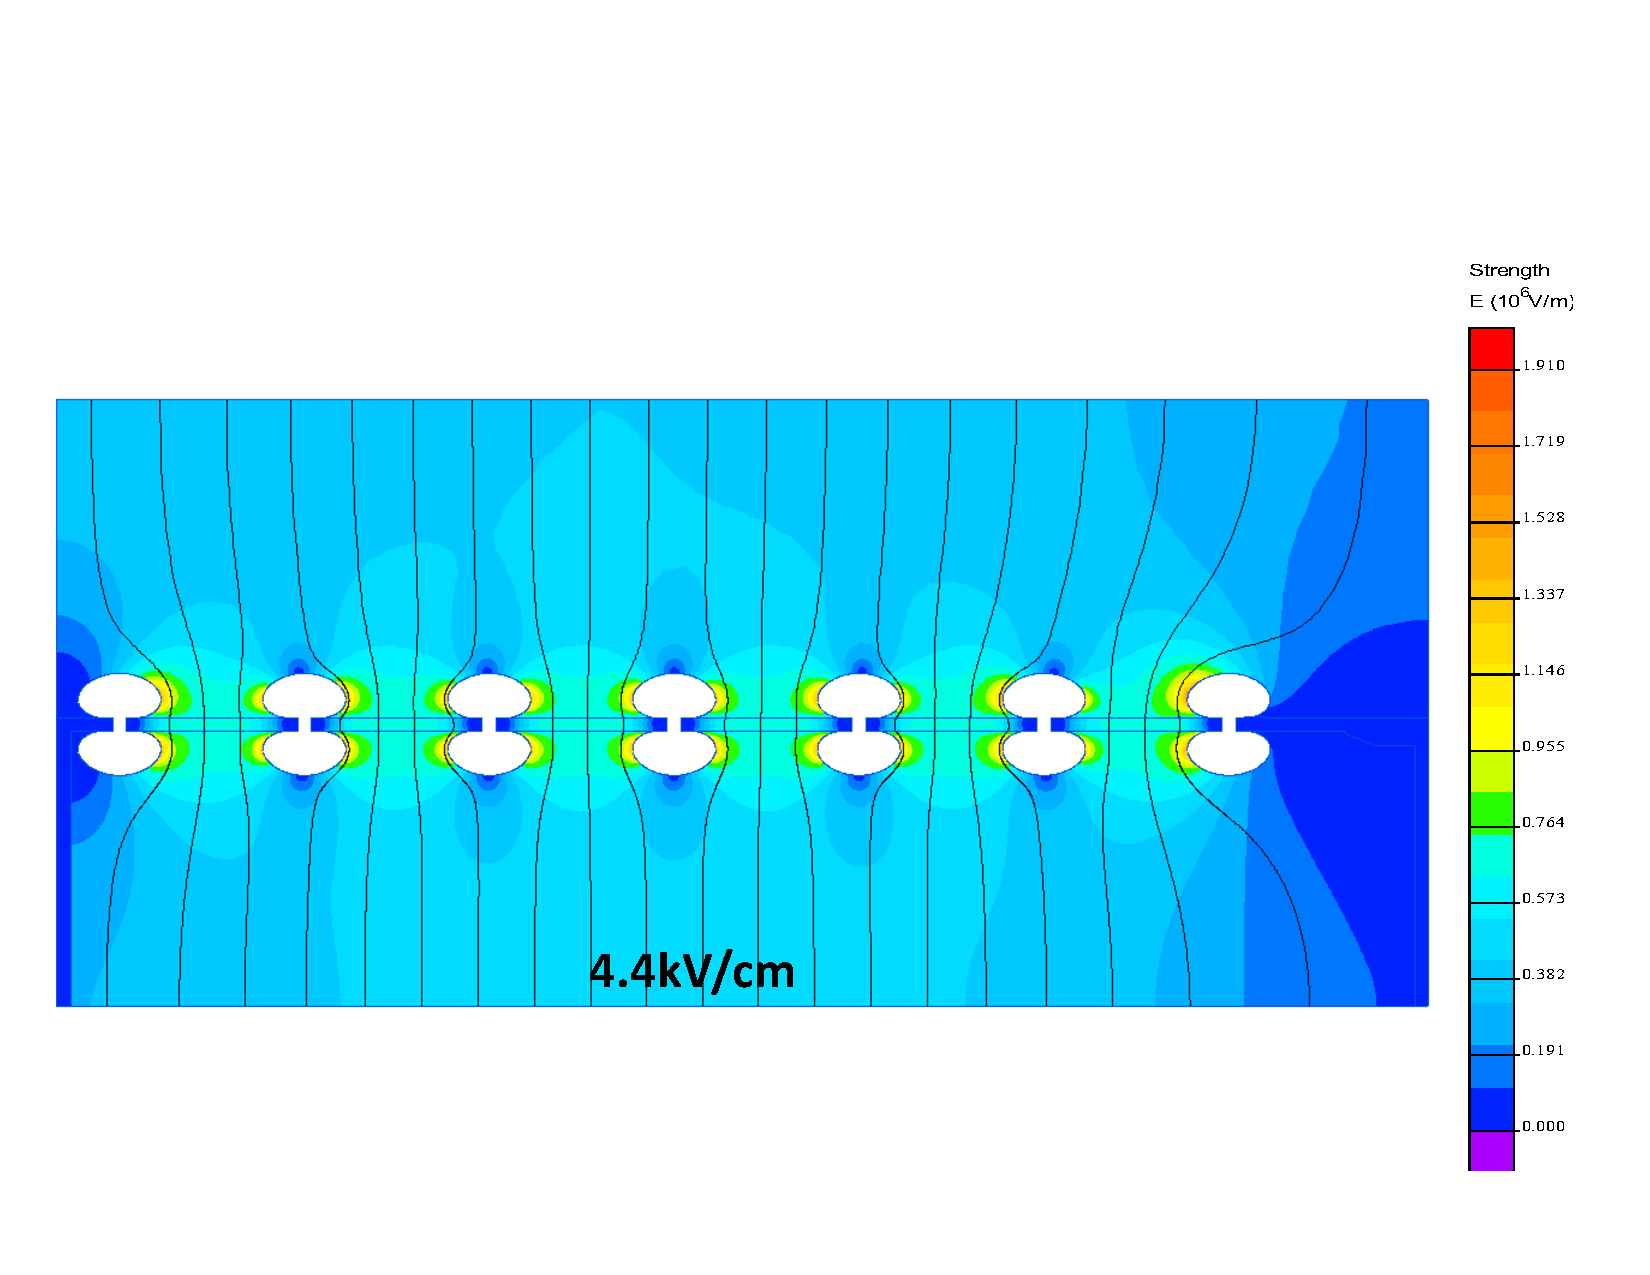
\includegraphics[width=0.85\textwidth]{beamplug_ring1.pdf}
\end{cdrfigure}

\begin{cdrfigure}[Beam plug electrode]{beamplug_ring2}{Electric field calculation near the vicinity of the electrode. The shape of the ring minimizes the high field region near the joints between the electrode, LAr, and composite shell. The field is well below the 30 kV/cm limit in all regions.}
  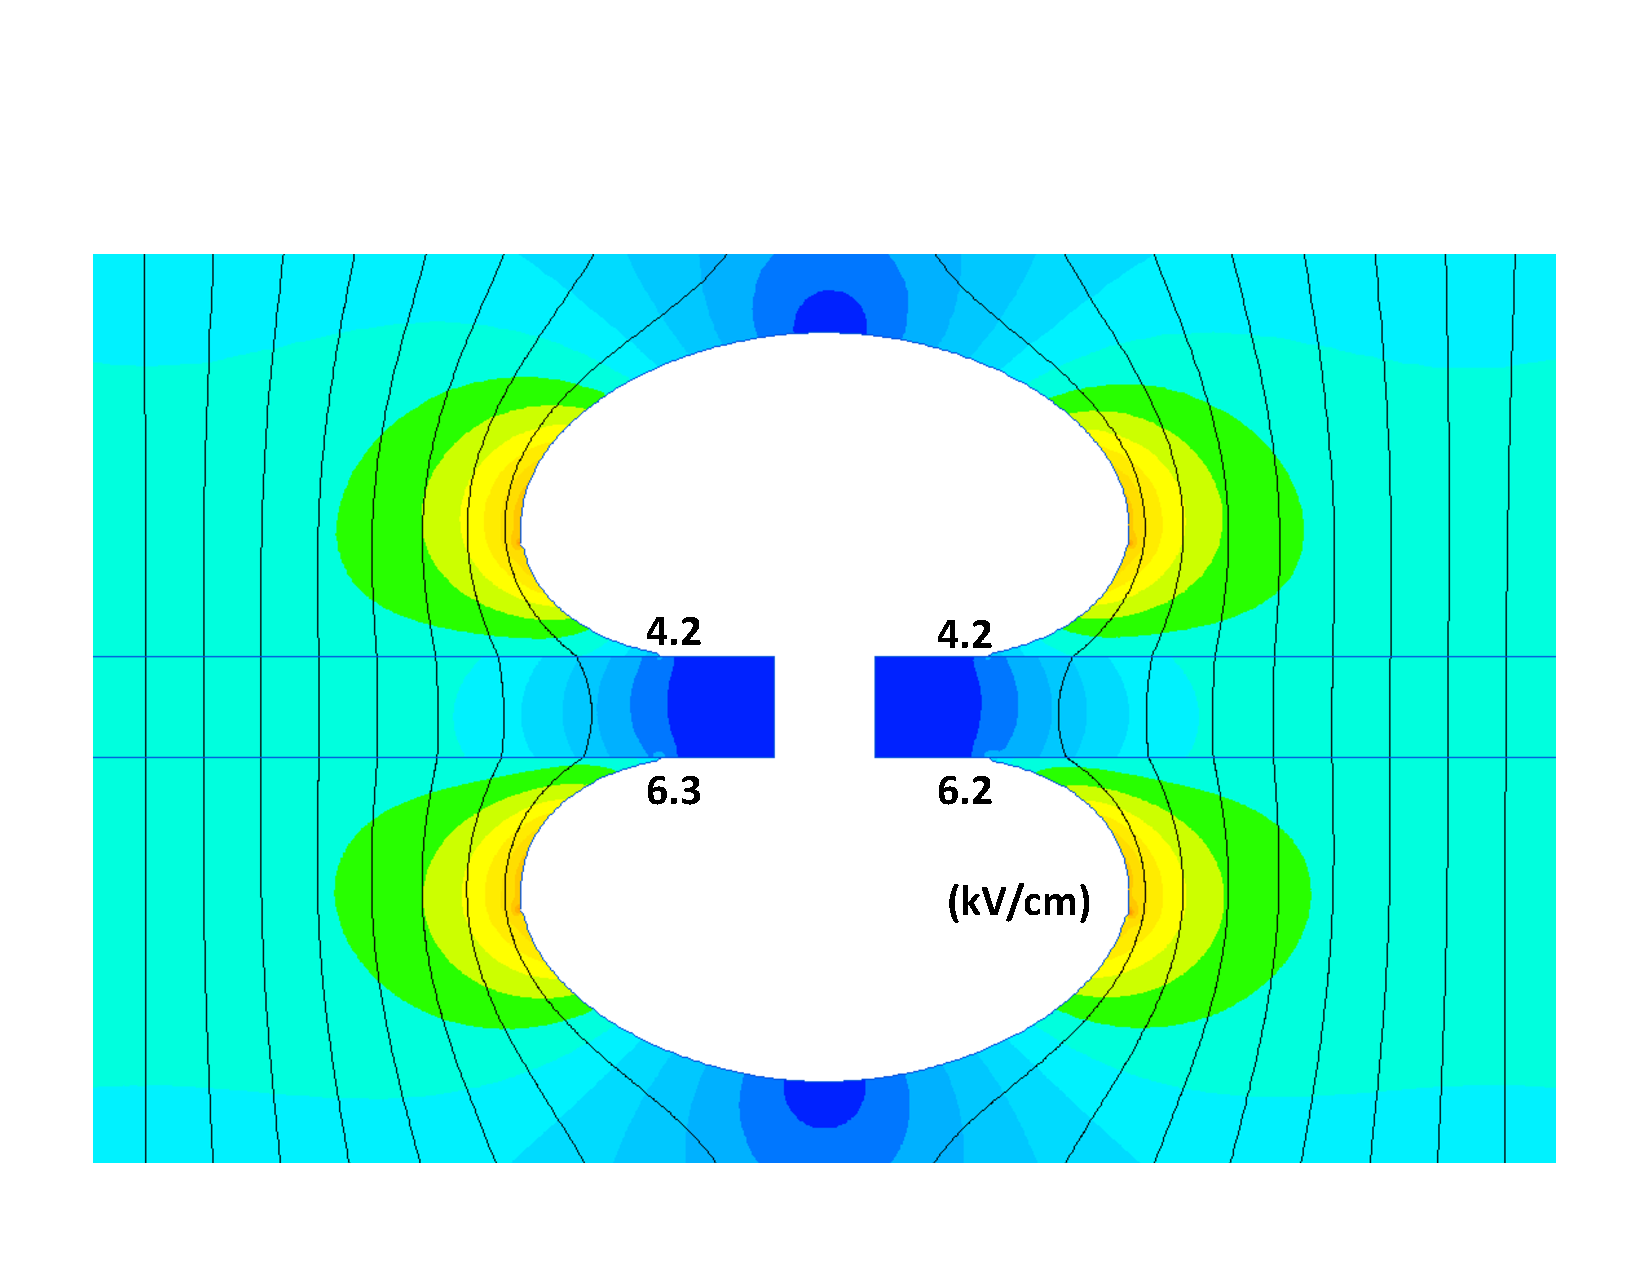
\includegraphics[width=0.5\textwidth]{beamplug_ring2.pdf}
\end{cdrfigure}

The beam plug is installed between the field cage and primary membrane where the charged particle beam enters the cryostat. Its main function is to displace about 45 cm of passive LAr layer in that region to allow the particle beam to enter the active TPC region with minimal upstream material interactions. The beam plug is mounted onto one of the field cage support structures as shown in Figures~\ref{fig:beamplug-fc} and~\ref{fig:beamplug-fc2}. The support structure is designed with sufficient  strength and stiffness to support the weight of the beam plug.
\begin{cdrfigure}[Beam plug to CPA connection]{beamplug-fc}{Beam plug to field cage interface.}
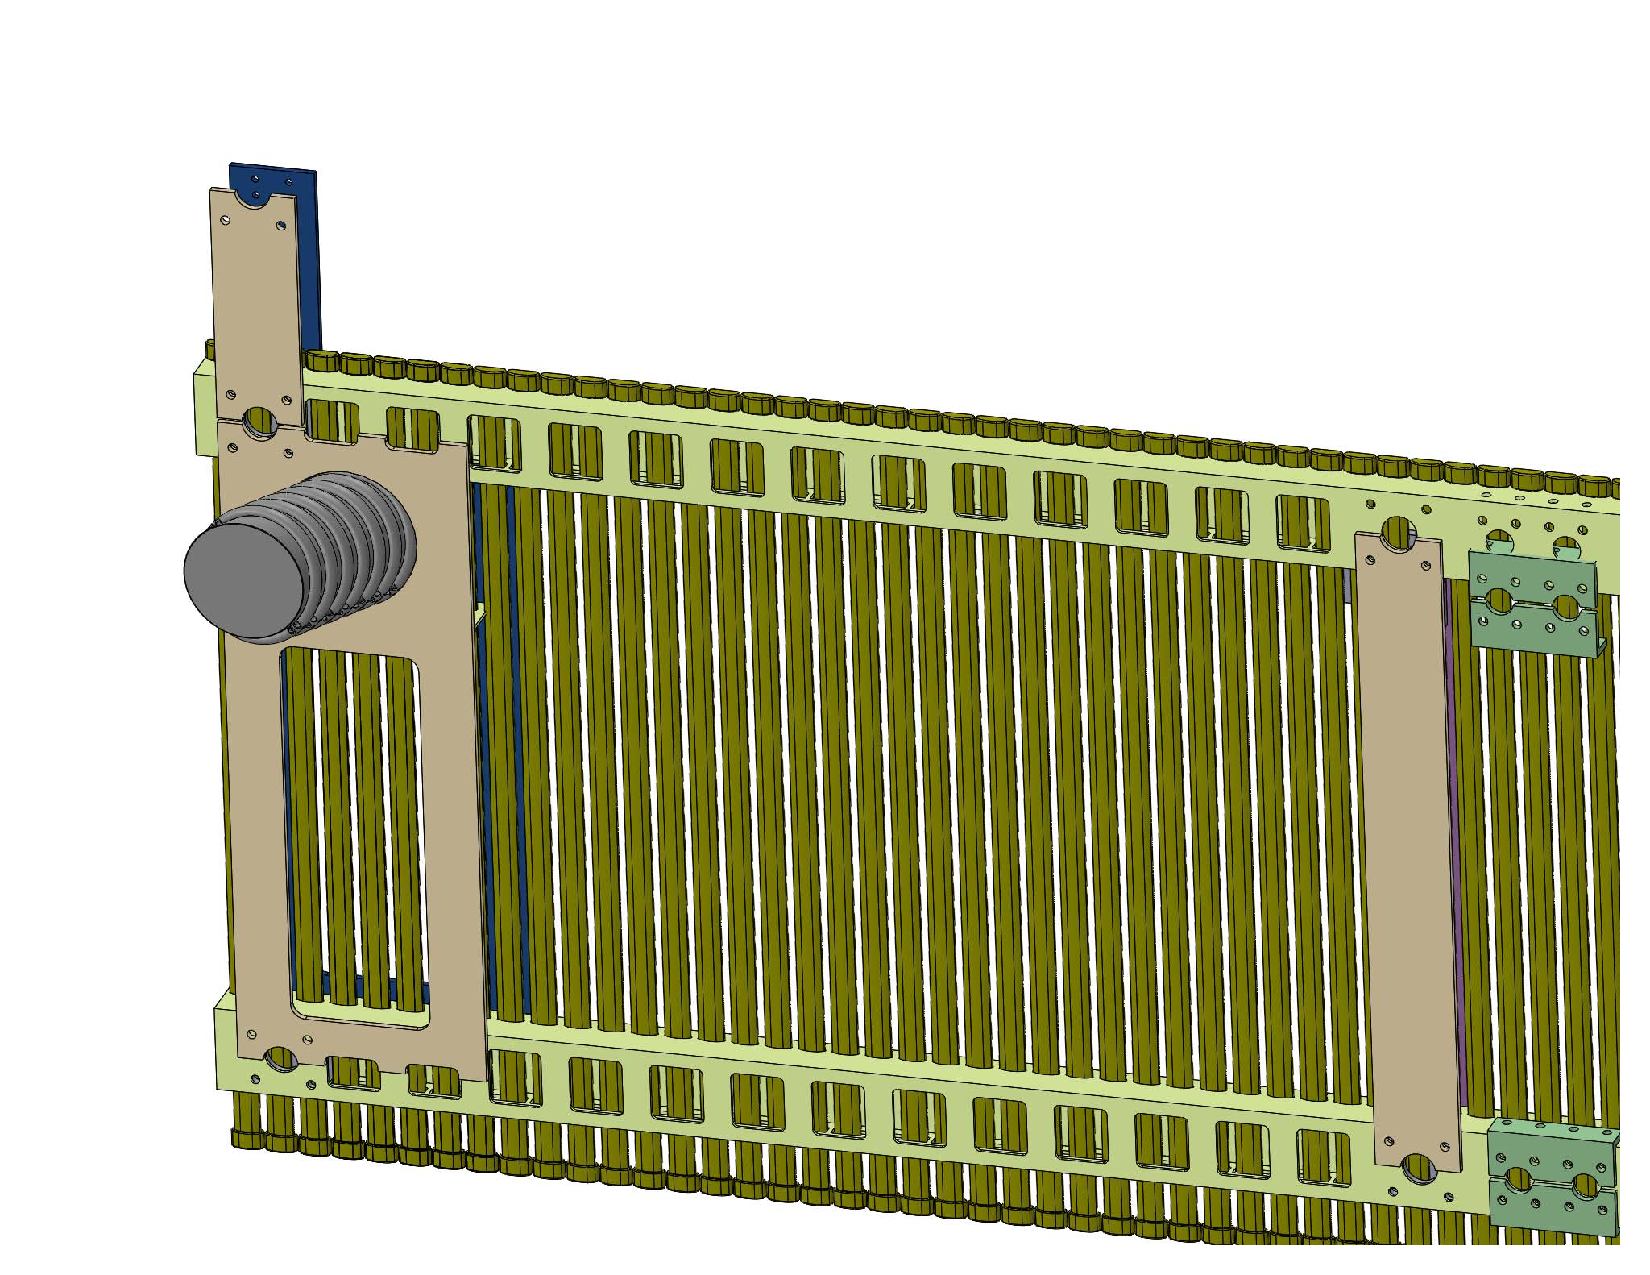
\includegraphics[width=0.75\linewidth]{beamplug-fc.pdf}
\end{cdrfigure}
\begin{cdrfigure}[Beam plug to CPA connection]{beamplug-fc2}{Cutaway sideview of the beam plug to field cage interface.}
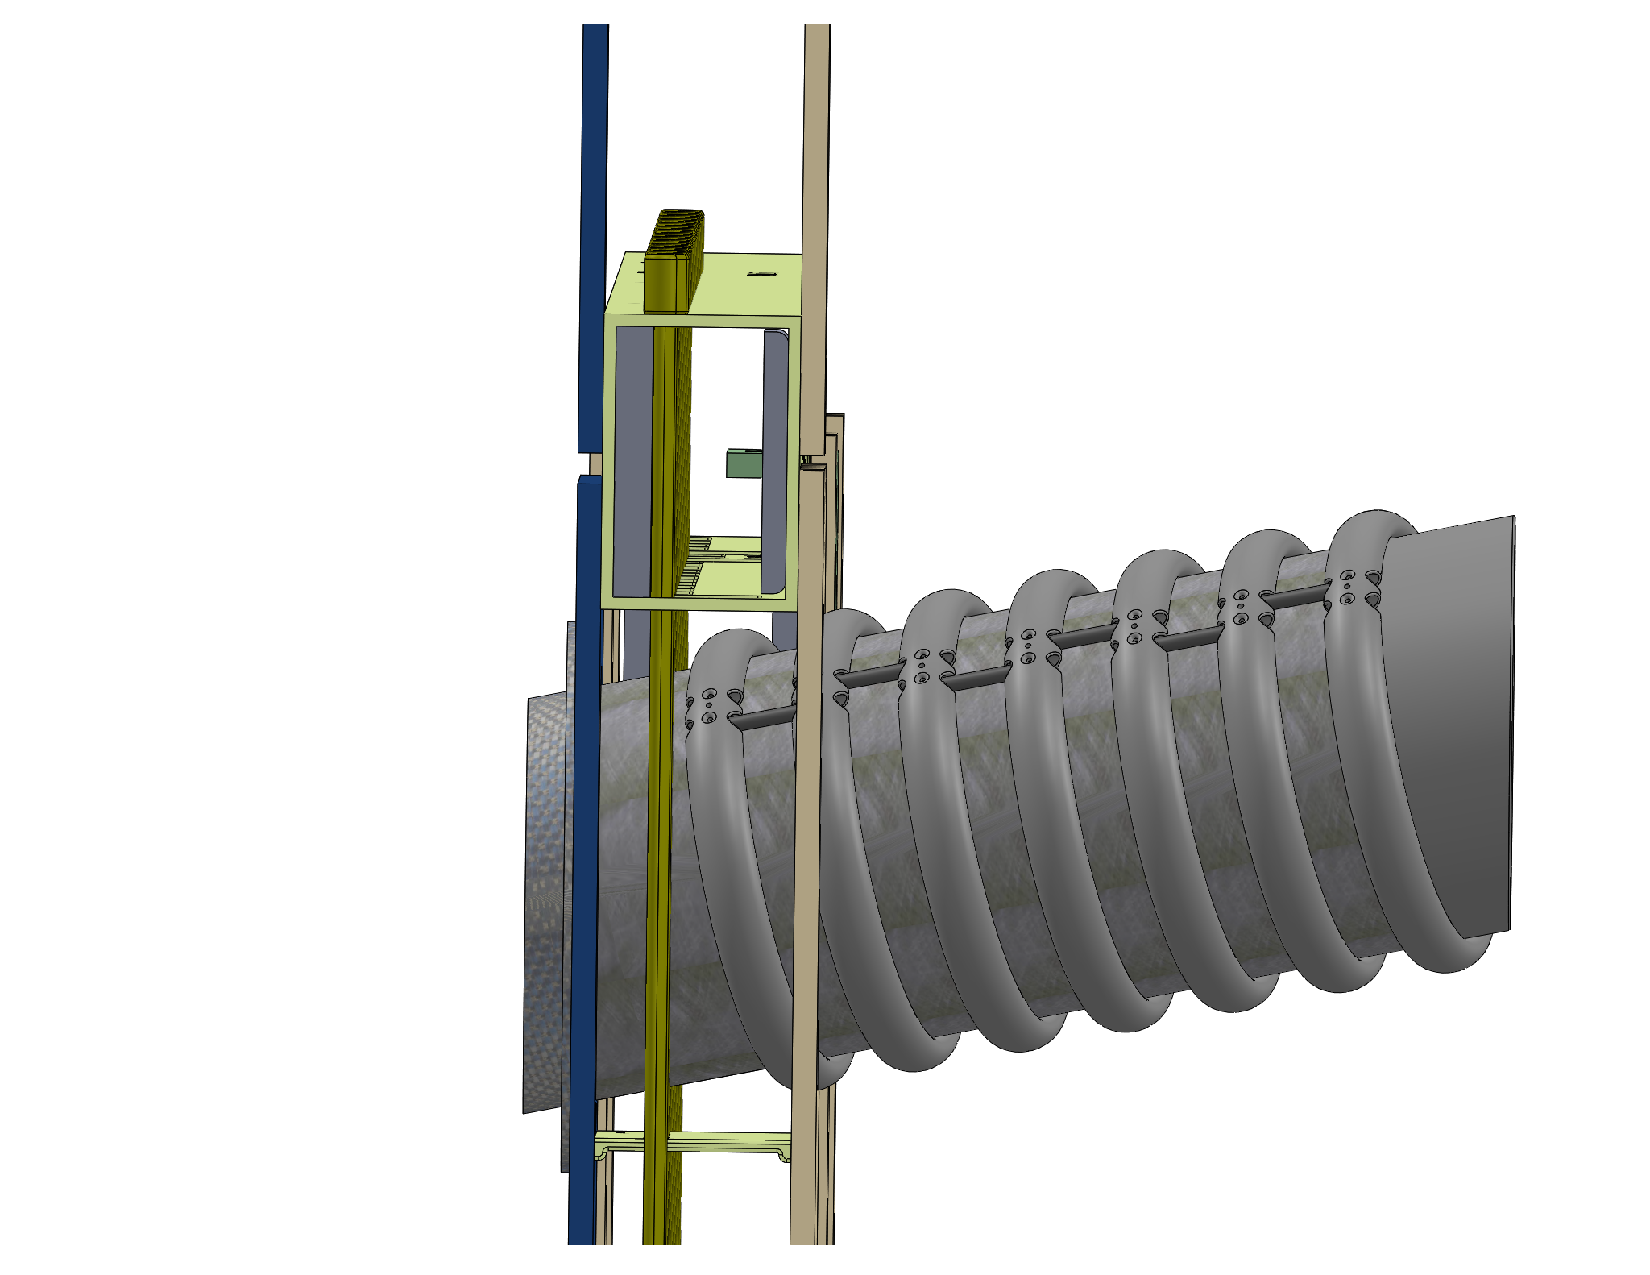
\includegraphics[width=0.5\linewidth]{beamplug-fc2.pdf}
\end{cdrfigure}


\paragraph{Field cage resistor divider chain with beam plug}
The resistor divider chain of the beam plug is tied to the main field cage profile. To maintain the 3 kV voltage drop across all field cage profiles, a second resistor divider board is added in parallel to the nominal board for the first 5 field cage profiles closest to the CPA. This modification is only needed for the field cage panel with the beam plug attached. The circuit diagram for the proposed scheme and the resistor values are shown in Figure~\ref{fig:beamplug_resistordivider}.
\begin{cdrfigure}[Beam plug resistor divider chain]{beamplug_resistordivider}{The resistor divider circuit for the end-wall field cage panel with the beam plug. The proposed resistor values for the main, parallel divider boards, and the beam plug are given in the tables.}
  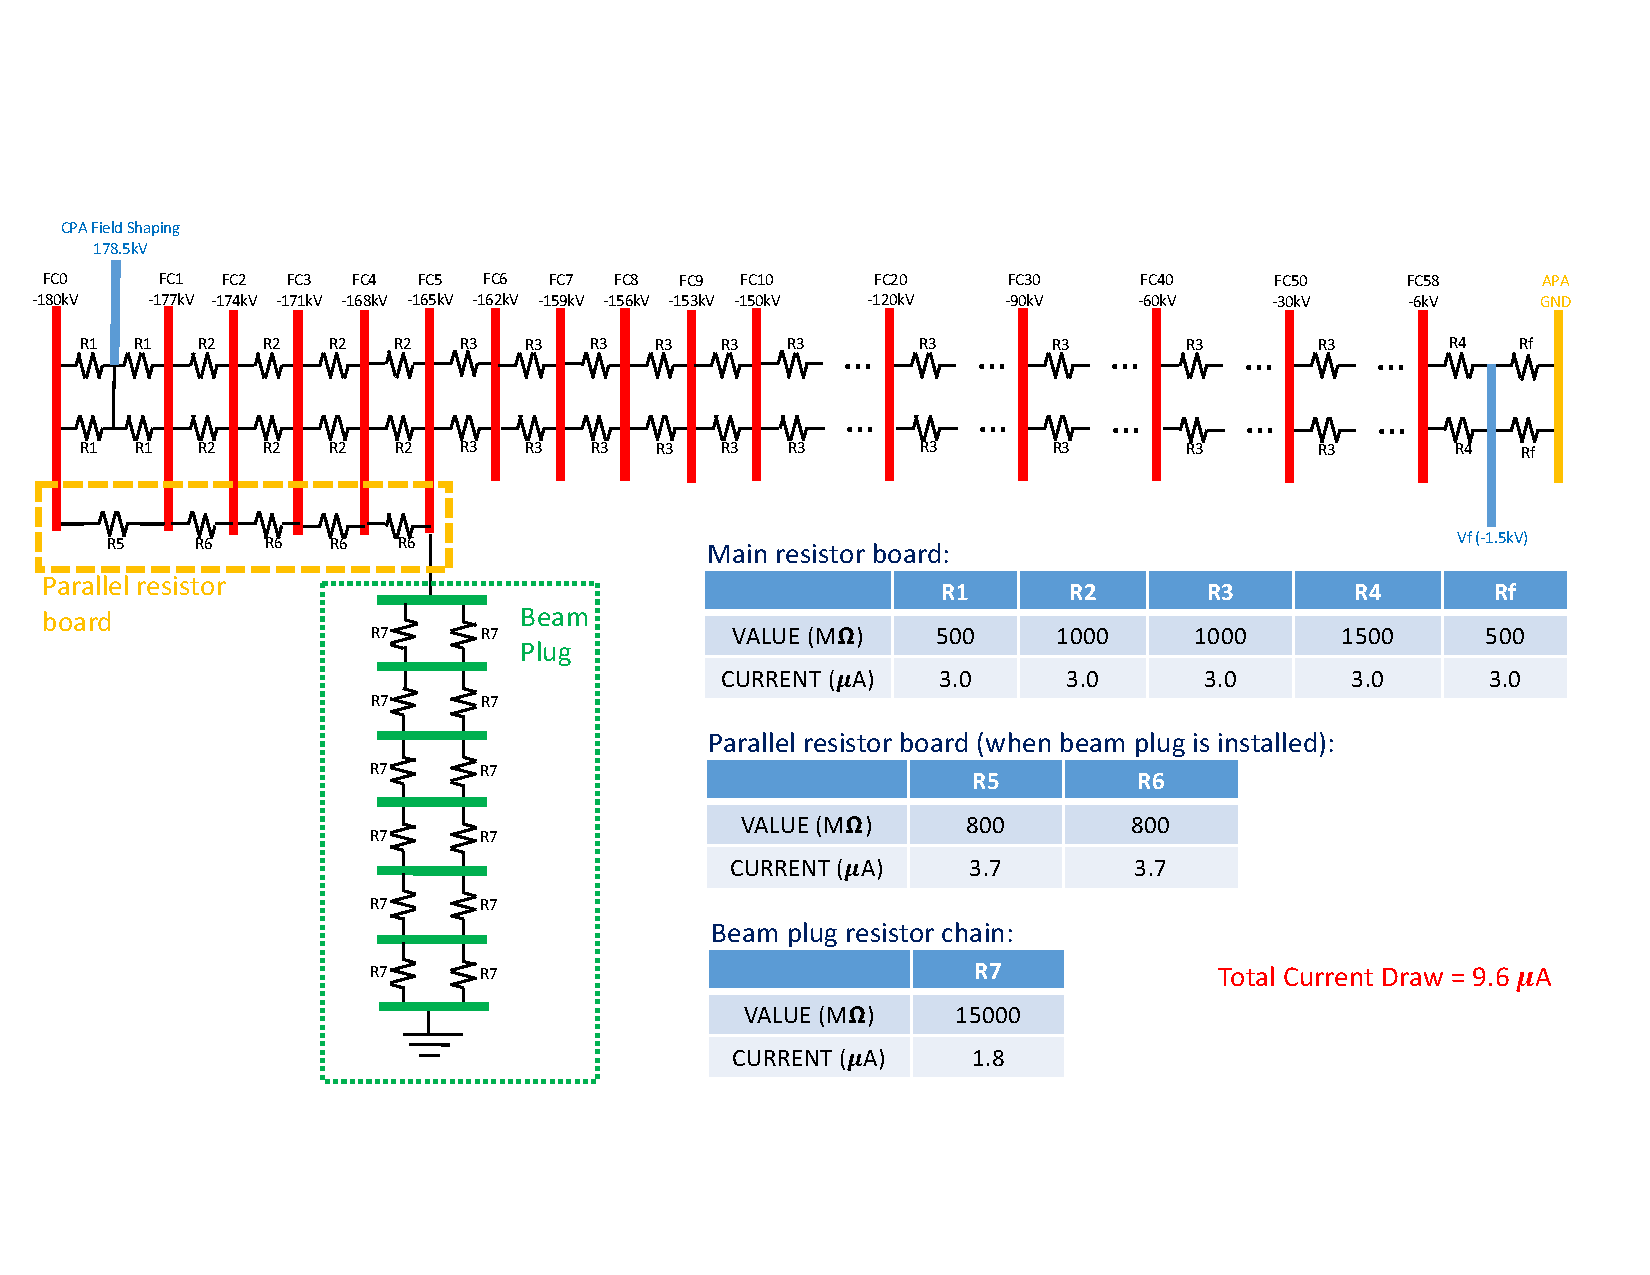
\includegraphics[width=0.85\textwidth]{beamplug_resistordivider.pdf}
\end{cdrfigure}
